\section{Primeras pruebas en MATLAB}

Desarrollado todo el fundamento teórico detrás del estudio que se está realizando y con el que se está tratando de conocer si mediante torsión de las palas de una turbina eólica se obtiene más energía, menos o la misma que si no se torsionasen, se debe avanzar y comenzar a hacer cálculos empíricos. \\

Estos cálculos y representaciones se realizarán mediante MATLAB, de la manera más ordenada y arbitraria posible. Con esto se busca la manera más simple de poder modificar las variables más sencillas que envuelven a los cálculos, para así poder cambiarlas a placer. \\

Algunas variables como, $L$, $\Theta_1$, $\Theta_i$  o $u$ deben ser establecidas por el propio estudiante, dando así un mayor juego a la amplitud de resultados posibles. \\

Una de las variables con las que se va a trabajar es la velocidad del viento y en este trabajo se va a regir mediante la \textbf{Escala Beaufort} \cite{BeaufortScale2012}. Esta unió varias tablas creadas hasta la época haciéndola así las más completa y por ello es la que se usará.\\

A continuación se detalla un acortamiento de la misma ya que no todos sus datos son relevantes para el estudio:

\begin{figure}[H]
    \centering
    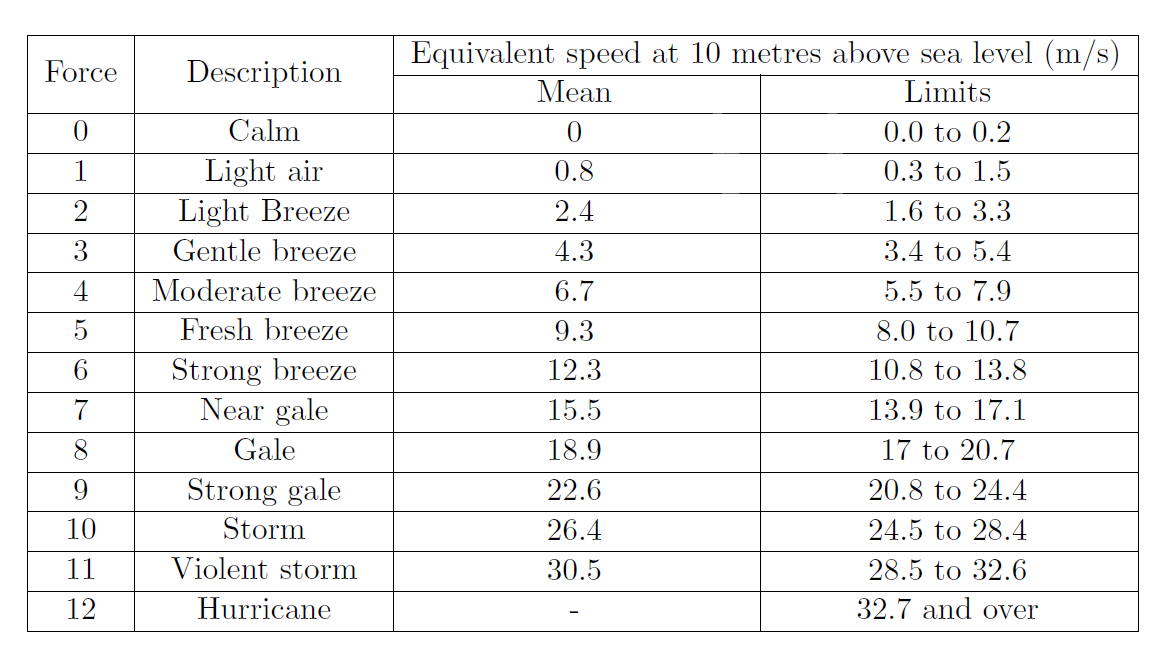
\includegraphics[width=1\textwidth]{images/Tabla Beaufort Efect.png}
    \caption{Escala Beaufort}
     Fuente: \cite{BeaufortScale2012}
     \label{tabla:escala_beaufort}
\end{figure}

% Please add the following required packages to your document preamble:
% \usepackage{multirow}
% \begin{table}[H]
% \centering
% \begin{tabular}{|c|c|cc|}
% \hline
% \multirow{2}{*}{Force} & \multirow{2}{*}{Description} & \multicolumn{2}{c|}{Equivalent speed at 10 metres above sea level (m/s)} \\ \cline{3-4} 
%   &                 & \multicolumn{1}{c|}{Mean} & Limits        \\ \hline
% 0  & Calm            & \multicolumn{1}{c|}{0}    & 0.0 to 0.2    \\ \hline
% 1  & Light air       & \multicolumn{1}{c|}{0.8}  & 0.3 to 1.5    \\ \hline
% 2  & Light Breeze    & \multicolumn{1}{c|}{2.4}  & 1.6 to 3.3    \\ \hline
% 3  & Gentle breeze   & \multicolumn{1}{c|}{4.3}  & 3.4 to 5.4    \\ \hline
% 4  & Moderate breeze & \multicolumn{1}{c|}{6.7}  & 5.5 to 7.9    \\ \hline
% 5  & Fresh breeze    & \multicolumn{1}{c|}{9.3}  & 8.0 to 10.7   \\ \hline
% 6  & Strong breeze   & \multicolumn{1}{c|}{12.3} & 10.8 to 13.8  \\ \hline
% 7  & Near gale       & \multicolumn{1}{c|}{15.5} & 13.9 to 17.1  \\ \hline
% 8  & Gale            & \multicolumn{1}{c|}{18.9} & 17 to 20.7    \\ \hline
% 9  & Strong gale     & \multicolumn{1}{c|}{22.6} & 20.8 to 24.4  \\ \hline
% 10 & Storm           & \multicolumn{1}{c|}{26.4} & 24.5 to 28.4  \\ \hline
% 11 & Violent storm   & \multicolumn{1}{c|}{30.5} & 28.5 to 32.6  \\ \hline
% 12 & Hurricane       & \multicolumn{1}{c|}{-}    & 32.7 and over \\ \hline
% \end{tabular}
%     \caption{Escala Beaufort}
% \end{table}


\subsection{¿Cuál es la torsión óptima?}

Previo a obtener resultados usando aerogeneradores con características reales como el tamaño de las aspas, se procede a probar un caso estándar en el que se presenta un ángulo de cabeceo establecido y estándar, por ejemplo 2$^{\circ}$.

En un primer momento se pensó hacer un ejemplo en el que sin ángulo de cabeceo se demostrase la importancia de la torsión con respecto a la obtención de energía. Pero como se comentó en el Desarrollo teórico, es necesario contar con una pala realista para que se genere una fuerza de sustentación y así generar energía. \\

Además, estableciendo un ángulo de cabeceo estático también es posible demostrar la importancia de la torsión como efecto y cuantitativamente.\\

Se procede a estudiar un primer ejemplo, este está generado para velocidades de viento en la escala de Beaufort de entre 0 y 8 de fuerza:

\begin{figure}[H]
    \centering
    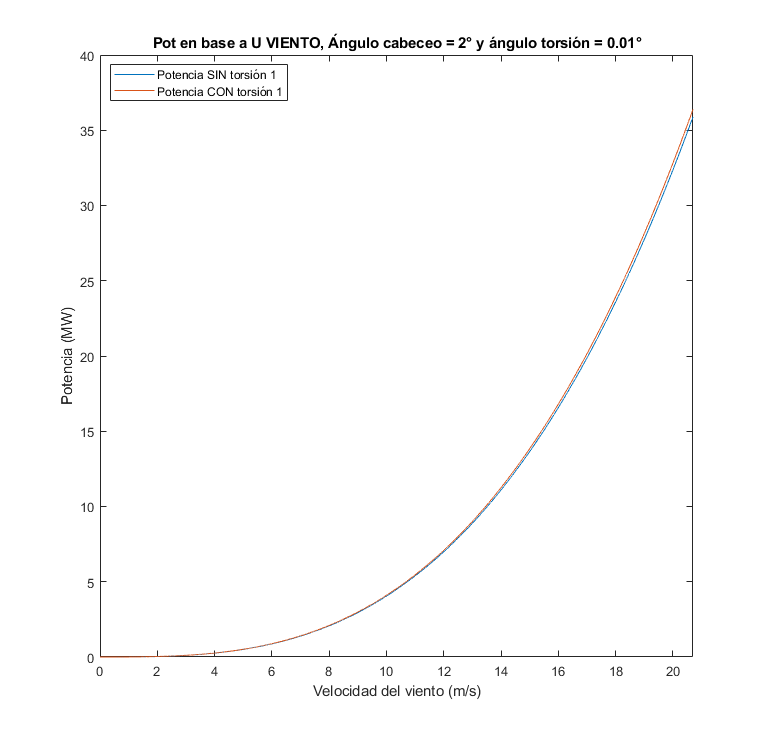
\includegraphics[width=1\textwidth]{images/0-8beau torsion.png}
    \caption{Potencia obtenida con viento de entre 0 y 8 de fuerza según la escala Beaufort}
     \label{fig:0-8beaufort_torsion_ejemplo_inicial}
\end{figure}

Observando la Figura \ref{fig:0-8beaufort_torsion_ejemplo_inicial} se puede vislumbrar la pequeña diferencia que supone haber torsionado las palas únicamente 0.1$^{\circ}$ por segmento. Además, parece que en el caso de hacer zoom en la figura la diferencia entre las potencias cada vez es menor. Se observa de nuevo la potencia para el caso en el cual las fuerzas del viento varían entre 0 y 5:

\begin{figure}[H]
    \centering
    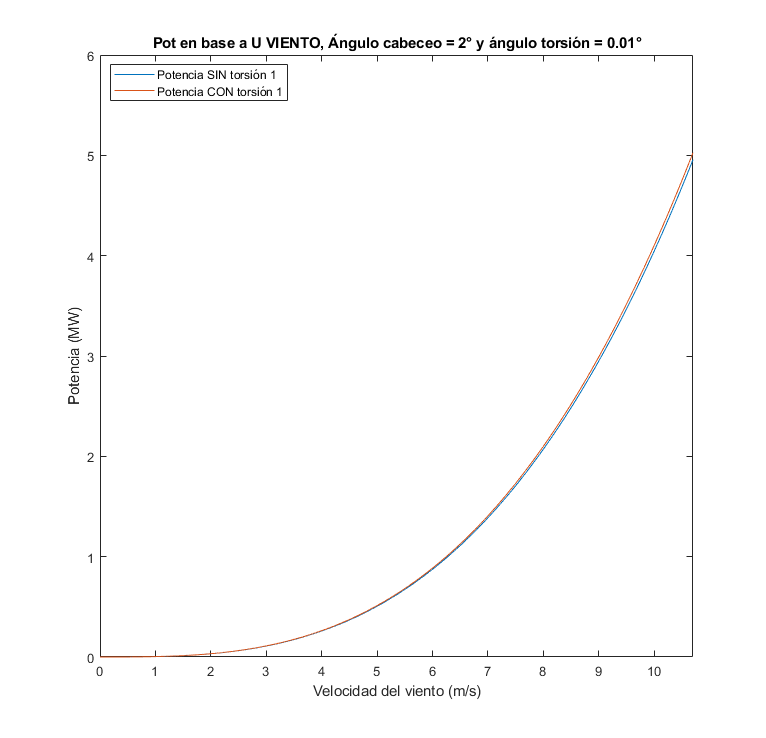
\includegraphics[width=1\textwidth]{images/0-5beau torsion.png}
    \caption{Potencia obtenida con viento de entre 0 y 5 de fuerza según la escala Beaufort}
     \label{fig:0-5beaufort_torsion_ejemplo_inicial}
\end{figure}

A simple vista pueden llegar a parecer la misma imagen, pero como se comentó, la Figura \ref{fig:0-5beaufort_torsion_ejemplo_inicial} es solo un zoom de la Figura \ref{fig:0-8beaufort_torsion_ejemplo_inicial}. Al aplicar el zoom se puede observar que las dos figuras presentan una forma casi idéntica, es por ello que se puede pensar que por mucho zoom que se realice, la diferencia entre ambas parece constante.\\

Se realiza el análisis de la eficiencia basándonos en las anteriores figuras para comprobar si la hipótesis planteada resulta ser correcta.\\

\subsection{Resultados usando el Aerogenerador SWT-6.0-154\cite{Siemens2022} de Siemens}

En este caso y utilizando un aerogenerador del que se conocen ciertas variables y factores que se han tenido en cuenta en este trabajo, se procede a obtener la potencia.\\

Se trata de un aerogenerador de grande dimensiones, es por ello que el \textit{CP} usado debe ser un valor entre 0.3 y 0.4, este valor lo establece el diseño del aerogenerador y al estar trabajando con un sistema inmaculado y en condiciones perfectas se usará 0.4 como valor.\\




En la anterior figura se puede observar la potencia que obtiene la pala que se ha definido si se le presentasen vientos vivos de entre 8 y 10 m/s y una torsión de 0.04$^{\circ}$ por segmento, lo cual puede parecer una variación baja teniendo en cuenta la longitud de la pala, pero no es así.\\